\documentclass[nonacm=true, language=french, language=english]{acmart}

%%%% PREAMBULE MAIN FILE %%%%

%%% INFORMATIONS %%%

% last update 04/2022

%%% CONDITIONNING %%%




\usepackage{ifthen}

% \newcommand\documentisfrench{}
\newcommand\fr[2]{\ifthenelse{\isundefined{\documentisfrench}}{#2}{#1}}

% \newcommand\documentisbeamer{}
\newcommand\ifbeamer[2]{\ifthenelse{\isundefined{\documentisbeamer}}{#2}{#1}}

% \newcommand\documentissansserif{}
\newcommand\sans[2]{\ifthenelse{\isundefined{\documentissansserif}}{#2}{#1}}

%%% FILES %%%

%%%% PREAMBULE PACKAGES FILE %%%%

%%% FONTS %%%
\usepackage[T1]{fontenc}
\usepackage[utf8]{inputenc}

\fr{
  \usepackage[french]{babel}
}{}

\usepackage{CJKutf8}            % chinese, japanese, corean
%\usepackage{numprint}          % pretty digits

%% fourrier
%\usepackage{fourier}
%\usepackage[scaled=0.875]{helvet}
%\usepackage{courier}

%% sans serif
\sans{
  \usepackage{cmbright}
  \renewcommand{\familydefault}{\sfdefault}
}{}



%%% MISE EN PAGE %%%
\ifbeamer{}{
  % \usepackage[a4paper]{geometry}
  % \geometry{hscale=0.7,vscale=0.8,centering}
}



%%% UTILITIES %%%
\usepackage{xcolor}         % couleur
\usepackage{xspace}         % espace automatique

\usepackage{xurl}           % Pour citer les adresses web
\usepackage{hyperref}       % Liens

\usepackage{stackengine}    % Empiler du texte

\usepackage[cache=false]{minted}         % inclusion de code

\usepackage{alltt}          % verbatim avec commandes

\usepackage{enumitem}       % listes



%%% TABLES %%%
\usepackage{multirow}       % fusion de ligne dans les tableaux
\usepackage{booktabs}       % Allows the use of \toprule, \midrule and \bottomrule in tables



%%% IMAGES %%%
\usepackage{graphicx} % inclusion des graphiques
\usepackage{wrapfig}  % Dessins dans le texte.

\usepackage{tikz}
\usetikzlibrary{cd}             % commutative diagrams via https://tikzcd.yichuanshen.de/
\usepackage[framemethod=TikZ]{mdframed}



%%% TREES %%%
\usepackage[linguistics]{forest}


\ifbeamer{
  %%%% PREAMBULE BEAMER FILE %%%%

% This template has been downloaded from:
% http://www.LaTeXTemplates.com

\mode<presentation> {

  % The Beamer class comes with a number of default slide themes
  % which change the colors and layouts of slides. Below this is a list
  % of all the themes, uncomment each in turn to see what they look like.

  % \usetheme{AnnArbor}
  % \usetheme{Antibes}
  % \usetheme{Bergen}
  % \usetheme{Berkeley}
  % \usetheme{Berlin}
  % \usetheme{Darmstadt}
  % \usetheme{Dresden}
  % \usetheme{Frankfurt}
  % \usetheme{Goettingen}
  % \usetheme{Hannover}
  % \usetheme{Ilmenau}
  % \usetheme{JuanLesPins}
  % \usetheme{Marburg}
  % \usetheme{Montpellier}
  % \usetheme{PaloAlto}
  % \usetheme{Pittsburgh}
  % \usetheme{Rochester}
  % \usetheme{Singapore}
  % \usetheme{Szeged}

  % \usetheme{default}       % rien (cadre carré)
  % \usetheme{Boadilla}      % bas3
  \usetheme{CambridgeUS}   % bas3 + haut2
  % \usetheme{Copenhagen}    % bas2
  % \usetheme{Luebeck}       % bas2 + haut2 (cadre/puces carré)
  % \usetheme{Madrid}        % = Boadilla
  % \usetheme{Malmoe}        % = Luebeck
  % \usetheme{Warsaw}        % bas2 + cardes ombre

  % As well as themes, the Beamer class has a number of color themes
  % for any slide theme. Uncomment each of these in turn to see how it
  % changes the colors of your current slide theme.

  % \usecolortheme{albatross}
  % \usecolortheme{beaver}
  % \usecolortheme{beetle}
  % \usecolortheme{crane}
  % \usecolortheme{dove}
  % \usecolortheme{fly}
  % \usecolortheme{lily}
  % \usecolortheme{orchid}
  % \usecolortheme{rose}
  % \usecolortheme{seagull}
  % \usecolortheme{whale}
  % \usecolortheme{wolverine}

  % \usecolortheme{dolphin}
  \usecolortheme{seahorse}

  % \setbeamertemplate{footline} % To remove the footer line in all slides uncomment this line
  % \setbeamertemplate{footline}[frame number] % To replace the footer line in all slides with a simple slide count uncomment this line

  % \setbeamertemplate{navigation symbols}{} % To remove the navigation symbols from the bottom of all slides uncomment this line

  % \setbeamercovered{transparent} % Fait apparaître les animations en grisé (utile pour la conception, mais peut être commenté lors de la remise du document final)

  % Pour utiliser une police à empattements partout
  % \usefonttheme{serif}

  % Pour rajouter la numérotation des frames dans les pieds de page
  % \newcommand*\oldmacro{}%
  % \let\oldmacro\insertshorttitle%
  % \renewcommand*\insertshorttitle{%
  % \oldmacro\hfill%
  % \insertframenumber\,/\,\inserttotalframenumber}


  % section/subsection
  \setbeamertemplate{section in toc}{%
    \quad ({\inserttocsectionnumber})~{\inserttocsection}%
  }
  \setbeamertemplate{subsection in toc}{%
    \quad\quad $\rhd$~{\inserttocsubsection} \\%
  }

  \setbeamertemplate{navigation symbols}{} % remove nav bar

}

% table des matieres (à paramétrer selon le document)
\setcounter{tocdepth}{2}

\newcommand\tocpage{
  \begin{frame}
    \tableofcontents[firstsection = 2 , currentsubsection]
  \end{frame}
}


%% arbres dans beamer (forest)
% permet d'utiliser onslide=<>{} pour animer les arbres (beamer)
\tikzset{onslide/.code args={<#1>#2}{
    \only<#1>{\pgfkeysalso{#2}}
  }}

\tikzset{
  invisible/.style={text opacity=0, draw opacity = 0},
  visible on/.style={alt=#1{}{invisible}},
  alt/.code args={<#1>#2#3}{%
    \alt<#1>{\pgfkeysalso{#2}}{\pgfkeysalso{#3}} % \pgfkeysalso doesn't change the path
  },
}
\forestset{
  visible on/.style={
    for tree={
      /tikz/visible on={#1},
      edge+={/tikz/visible on={#1}}}}}

}{}

%%%% PREAMBULE MACROS FILE %%%%


\PassOptionsToPackage{svgnames}{color}


% Espace automatique après un guillemet fermant
\fr{
  \renewcommand{\fg}{\fg\xspace}
}{}

%% parenthèses, crochets & accolades qui s'adaptent à la taille de ce qu'il y a à l'intérieur
\newcommand{\ap}[1]{\left(#1\right)}        % auto parenthesis
\newcommand{\ab}[1]{\left[#1\right]}        % auto bracket
\newcommand{\acb}[1]{\left\{#1\right\}}     % auto curly bracket


%% Puces pour les listes
\setitemize[1]{label=$\diamond$}
\setitemize[2]{label=$\circ$}
\setitemize[3]{label=$\star$}

\setenumerate[1]{label=\arabic*.}
\setenumerate[2]{label=\theenumi\arabic*.}
\setenumerate[3]{label=\theenumii\arabic*.}
\setenumerate[4]{label=\theenumiii\arabic*.}
% \setenumerate[2]{label=\alph*.}
% \setenumerate[3]{label=\roman*.}

% style d'item description
\renewcommand{\descriptionlabel}[1]{%
  \hspace\labelsep \upshape\bfseries \textit{#1}%
}


% point median
\newcommand\ptm\textperiodcentered

%soulignement
\newcommand\ul\underline


% panneau attention
\newcommand\danger{
    \makebox[1em]{
        \makebox[0pt][s]{
            % \raisebox{.1em}
            {\footnotesize !}
        }
        \makebox[0pt]{
          \raisebox{-0.1em}
          {\color{red}\Large$\bigtriangleup$}
        }
    }
}


%% écrire une remarque
\newcommand{\rk}[1]{$\rhd$ \textbf{Remar\fr{que}{k}} \emph{#1} }
\newcommand{\qrk}[1]{$\rhd$ \emph{#1} } % quick remark : pas de texte


% encadre le texte passe en parametre sur toute la largeur de la page
\newcommand{\longbox}[1]{
    \begin{center}\fbox{\parbox{\textwidth}{
        #1
    }}\end{center}
}


%% signatures
% manuscrite + nom dessous
\newcommand{\sign}
{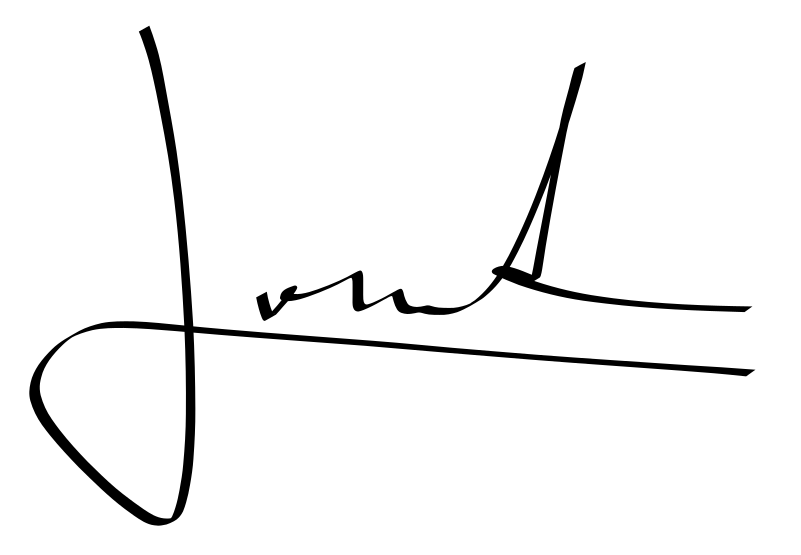
\includegraphics{preambule/signature_rj_small.png}\\ Robin \bsc{Jourde}}
% manuscrite + nom aligné à droite
\newcommand{\rsign}{\begin{flushright}\sign\end{flushright}}
% nom
\newcommand{\qsign}{Robin \bsc{Jourde}}
% nom aligné à droite
\newcommand{\rqsign}{\begin{flushright}\qsign\end{flushright}}



% email
\newcommand{\mailto}[1]{\href{mailto:#1}{\texttt{#1}}}


%%% PACKAGES %%%
\usepackage{amssymb}
\usepackage{amsmath}
\usepackage{mathrsfs}
\usepackage{amsfonts}

\usepackage{amsthm}         % theoremes et preuves
\usepackage{bussproofs}     % preuves en déduction nat et autres règles

\DeclareMathAlphabet{\varmathbb}{U}{bbold}{m}{n} % mathbb pour les chiffres


%%% LETTRES GRECQUES %%%
\renewcommand\phi{\varphi}
\renewcommand\epsilon{\varepsilon}



%%% MACROS %%%
%% Ensembles gras
\newcommand\N{\mathbb N}
\newcommand\Z{\mathbb Z}
\newcommand\D{\mathbb D}
\newcommand\Q{\mathbb Q}
\newcommand\R{\mathbb R}
\newcommand\C{\mathbb C}
\newcommand\K{\mathbb K}
\newcommand\F{\mathbb F}
\newcommand\E{\mathbb E}
\renewcommand\P{\mathbb P}


%% chiffres gras
\newcommand\zero{\varmathbb 0}
\newcommand\one{\varmathbb 1}
\newcommand\two{\varmathbb 2}



%% Autres ensembles
\newcommand\0{\varnothing}

\newcommand\M{\mathscr M}
\newcommand\MnR{\M_n(\R)}
\newcommand\MnC{\M_n(\C)}
\newcommand\MnK{\M_n(\K)}

\newcommand\B{\mathcal B}
\newcommand\Cl{\mathscr C}
\newcommand\Fn{\mathscr F}

\newcommand\Sfrak{\mathfrak S}



%% Opérateurs classiques
\DeclareMathOperator\id{id}
\DeclareMathOperator\Vect{Vect}
\DeclareMathOperator\card{card}
\DeclareMathOperator\rg{rg}
\DeclareMathOperator\im{im}
\DeclareMathOperator\colim{colim}

%% Catégories
\newcommand\Set{\mathbf{Set}}
\newcommand\Yo{\!\text{\begin{CJK}{UTF8}{min}よ\end{CJK}}}
\newcommand\op{{\,^\text{op}}}
\newcommand{\cattxt}[2]{#1\mathbf{\textbf{-}#2}}
\newcommand{\nlab}[1]{\href{https://ncatlab.org/nlab/show/#1}{[\fr{voir sur le}{see on} nlab]}}

\DeclareMathOperator\st{st}
\DeclareMathOperator\ob{ob}
\DeclareMathOperator\Ran{Ran}
\DeclareMathOperator\Lan{Lan}
\DeclareMathOperator\Kl{Kl}
\DeclareMathOperator\Hom{Hom}

%% Divers

% equivalent
\newcommand{\eq}[1]{\underset{#1}{\sim}}

% fleche de limite
\newcommand{\tend}[2]{\underset{#1 \to #2}{\longrightarrow}} 

% definition d'une fonction
\newcommand{\func}[4]{
    \ \begin{array}{|lll}
        #1 &\longrightarrow& #2 \\
        #3 &\longmapsto& #4
    \end{array}
}

%bijection
\newcommand\bij{\xrightarrow{\sim}}

%autres fleches
\newcommand{\xto}[1]{\xrightarrow{#1}}
\newcommand\too{\multimap}

\newcommand\from{\leftarrow}
\newcommand\mapsfrom{\mathrel{\reflectbox{\ensuremath{\mapsto}}}}

%d rond
\newcommand\drond{\partial}

% carre de fin de preuve
\renewcommand\qedsymbol{$\square$}
\newcommand\cqfd{\begin{flushright}\qedsymbol\end{flushright}}

%% Theoremes FR
\theoremstyle{plain}
\newtheorem{thm}{\fr{Théorème}{Theorem}}[section]
\newtheorem{lem}[thm]{Lemm\fr{e}{a}}
\newtheorem{cor}[thm]{Corolla\fr{ire}{ry}}
\newtheorem{prop}[thm]{Proposition}
\newtheorem{obj}{\fr{Objectif}{Goal}}


\theoremstyle{definition}
\newtheorem{ex}[thm]{Ex\fr{e}{a} mple}
\newtheorem{dfn}[thm]{D\fr{é}{e} finition}
\newtheorem{nota}[thm]{Notation}

\theoremstyle{remark}
\newtheorem{rem}[thm]{Remar\fr{que}{k}}

%% Disjonctions de cas
\newenvironment{disjonction}{\begin{enumerate}[label=\textbf{Cas\fr{e}{}  \arabic*.}]}{\end{enumerate}}


\usepackage{listings}
\lstset{
    basicstyle=\ttfamily\footnotesize,
    captionpos=b,
    numberstyle=\tiny\color{gray},
    numbers=left,
}

\setcopyright{none}

\author[R. Jourde]{Robin Jourde}
\affiliation{%
  \institution{École Normale Supérieure de Lyon}%
  \country{France}%
}
\email{Robin.Jourde@ens-lyon.fr}
\author{Supervised by Sam Lindley}
\email{Sam.Lindley@ed.ac.uk}
\author{Daniel Hillerström}
\email{Daniel.Hillerstrom@ed.ac.uk}
\affiliation{%
  \institution{The University of Edinburgh}%
  \country{United Kingdom}%
}

\renewcommand\shortauthors{Robin Jourde}


\title[M1 Intership Report]{M1 Internship Report : Effect Typing for Links}
\subtitle{2 May 2022 -- 22 July 2022, The University of Edinburgh}

\date{2 May 2022 -- 22 July 2022}

\begin{document}


\begin{abstract}
  This paper is the report of my internship at the School of Informatics of the University of Edinburgh with Sam Lindley and Daniel Hillerström from 2 May 2022 to 22 July 2022.
  Effect handlers are a language feature that is becoming more and more widespread. They allow the user to define and compose many functionalities from exceptions to concurrency and probabilistic programming.
  Links is an experimental tierless functional language for the web, mainly developed in the University of Edinburgh. Among its numerous features, Links supports effect handlers.
  The goal of my intership was to improve the effect typing system of Links, allowing aliases, avoiding pollution and allowing polymorphic operations.
\end{abstract}


\maketitle

\tableofcontents


\section{Introduction}

\section{Links}

\begin{fquote}[Links website (\url{https://links-lang.org/})]
 Links is a functional programming language designed to make web programming easier.
\end{fquote}

Links \cite{} is a tierless functional programming language for the web developed at the University of Edinburgh. Typical web development involves the manipulation of several \emph{tiers} which means several, sometimes really different, programming languages :
\begin{itemize}
  \item the server side written in Python or Java for instance
  \item the client side in JavaScript and HTML/CSS
  \item the database queries in SQL
\end{itemize}
This is neither elegant nor really practical and prevents easy binding between different parts of the program that need to communicate data. It can cause \emph{impedance mismatch}, ie situations where the objects required by the server do not match what the database provide and vice versa.

Links avoids these by providing the programmer one single language for each tier (HTML/CSS are still needed) that is compiled into bytecode for the server, JavaScript for the client and SQL for the queries.

Links also supports numerous useful features including
\begin{itemize}
  \item polymorphic variants
  \item regular expressions
  \item session types
  \item row typing
  \item effect handlers (see \ref{sec:handlers})
\end{itemize}
It is used as an experimental language by researchers to try out new ideas and what could be future widespread programming languages features.

Links is strict, statically typed and use a Hindley-Milner type system as well as a Rémy style row typing system \ref{sec:row-typ} \cite{}. Its syntax is inspired from JavaScript and ML. Its compiler \cite{} is written in OCaml.

\qrk{In appendix \ref{sec:tech}, the reader could find some technical points on Links syntax and semantics that are not worth it to develop here. He is invited to look at it whenever needed.}

\section{Effect handlers}
\label{sec:handlers}

In functional programming, functions are seen as black boxes that takes an input and computes an output. Though this view of \emph{pure} functions is convenient and pleases $\lambda$-calculus fans, it fails to accurately represent what real programming is. Computations interact with the outer world by many means :
\begin{itemize}
  \item input/output
  \item concurrency
  \item exceptions
  \item choice and non determinism
  \item ...
\end{itemize}
The ``outer world'' here stand for anything that is not the pure computation, from memory, other threads and user interaction to the evaluation context itself.
These interactions not taken into account by the black-box model are called \emph{effects}.

Gordon Plotkin and Matija Pretnar \cite{} introduced a construct that allow \emph{composable} and \emph{customisable} user-defined interpretation of effects : \emph{effect handlers}. They give the programmer direct access to the context, in the form of a first class continuation, often called \emph{resumption}.

Effect handlers can be seen as a generalisation of exception handlers. One can perform an effect in the same way as one could raise an exception and this will transfer the flow control to a handler. It is given the delimited continuation between the point where the effect is performed and where it is handled and can use it
\begin{description}
  \item[0 times] and act as an exception handler
  \item[once] (linear handler)
  \item[twice or more] (non-linear handler) to simulate a choice for instance
\end{description}


\subsection{Syntax and usage}

We give the Links syntax alongside with usage of effect handlers and operations. All examples in this report are written in Links.

Inside any segment of code, one can invoke an operation \verb'Op' with payload \verb'p' writing \verb'do Op(p)'. This has to be scoped into a handler of this operation. It will take the payload and the resumption and decide what to do.

\begin{lstlisting}[caption=Handler,label=lst:handler]
  handle ( code ) {
    case <Op(p) => r> -> ...
    case x -> ...
  }
\end{lstlisting}

Listing \ref{lst:handler} give the syntax for a handler for \verb'Op', \verb'code' being the code that can perform the operation. When the operation is invoked, the right hand side of line 2 is executed with \verb'p' the payload and \verb'r' the resumption bound in context. When \verb'code' returns a value, line 3 is executed with \verb'x' bound to that value.

If the handler gives the resumption a value \verb'v', it acts as if \verb'do Op(p)' returned the value \verb'v'. If the payload has type \verb't' and \verb|v| has type \verb|t'|, we say that \verb|Op| has type \verb|t => t'|.

The type system keeps track of what effects can be performed. A function from type \verb|a| to \verb|b| which can performs operations \verb|Op1: t1 => t1'|, \dots, \verb|Opk:tk => tk'| will have type \verb+(a) {Op1:t1 => t1', ..., Opk:tk => tk'}-> b+.


\subsection{Examples}

\subsubsection{A first exception handler}
\label{sec:first-except-handl}

~

\begin{lstlisting}[caption=Fail invocation]
  sig assert_positive : (Int) {Fail:() => Zero|_}-> Int
  fun assert_positive(x) {
    if (x>0) x else absurd(do Fail)
  }
\end{lstlisting}

This first example shows a function \verb|assert_positive| that takes an integer and returns it only if it positive, else, it raises the effect \verb|Fail| (for details on \verb|absurd| and the \verb|Zero| type, see \ref{sec:tech:zero}). This is the simplest example when one operation is invoked with no payload.

\begin{lstlisting}[caption=maybe handler, label=lst:mb-h]
  sig maybe : (() {Fail:() => Zero|e}~> a) {Fail{_}|e}~> Maybe(a)
  fun maybe(m) {
    handle(m()) {
      case <Fail> -> Nothing
      case x -> Just(x)
    }
  }
\end{lstlisting}

This operation can be handled by handler \ref{lst:mb-h}. This is actually an exception handler since the resumption is not used in the right hand side (and thus can be omitted in the left hand side). The \emph{effect signature} is \verb|{Fail: () => Zero}|, that means there is only one operation called \verb|Fail| that will be handled.

When the operation \verb|Fail| is invoked, the handler directly returns a value, here \verb|Nothing|. When the computation returns a value, the handler will return that value, embedded in the \verb|Maybe| type (on \verb|Maybe| type, see \ref{sec:tech:maybe}).

The function \verb|maybe| will take a computation that can perform the effect \verb+{Fail: () => Zero|e}+ ie the operation \verb|Fail| and possibly other effects, captured by the row variable \verb|e|, and returns something of type \verb|a|. It will execute this computation, performing effects from \verb|e| that should be handled by another handler at some point. In the end, it returns a value of type \verb|Maybe(a)|.

The \verb|Fail{_}| in the effect row indicates a polymorphic presence for the operation. Roughly it means that the operation can or cannot be present after. This is needed since the effect type system enforces that all operations in a row are distinct. \verb|Fail| cannot belong to \verb|e| because of the effect row of the input computation.

\begin{lstlisting}
  sig h2g2 : () {Fail:() => Zero}~> Int
  fun h2g2 () {
    assert_positive( -6 * -7 )
  }
  sig h2g2' : () {Fail:() => Zero}~> Int
  fun h2g2' () {
    assert_positive( -6 ) * -7
  }
\end{lstlisting}

We can then use the \verb|maybe| function to handle the failures in functions \verb|h2g2| and \verb|h2g2'| :

\begin{lstlisting}[caption=Links console]
  links> maybe ( h2g2 ) ;
  Just(42) : Maybe (Int)
  links> maybe ( h2g2' ) ;
  Nothing : Maybe (Int)
\end{lstlisting}

\section{Typing}

\subsection{Row Typing}
\label{sec:row-typ}


\subsection{Bidirectional Typing}



\section{Contributions}

\subsection{Effect Aliases}

\subsection{Fresh Labels}

\subsection{Polymorphic Operations}




\bibliographystyle{alpha}
\bibliography{biblio.bib}


\appendix

\section{Links technicalities}
\label{sec:tech}

Here are some technical points on Links syntax and semantics.

\subsection{Empty type}
\label{sec:tech:zero}
The empty type is \verb|Zero|. To destroy it, we use the following \verb|absurd| function.
\begin{lstlisting}
  sig absurd : (Zero) -> a
  fun absurd(x) {
    switch ( x ) {}
  }
\end{lstlisting}

\subsection{Option type}
\label{sec:tech:maybe}
Links has a builtin polymorphic option type \verb|Maybe| defined as below. An object of type \verb|Maybe(a)| is either \verb|Nothing| or \verb|Just(x)| where \verb|x| is of type \verb'a'
\begin{lstlisting}
  typename Maybe(a) = [| Nothing  | Just : a |]
\end{lstlisting}

\subsection{Function types}
Function types are written \verb|(a) {...}-> b|. The domain type is always embraced with parentheses. The braces contains an effect row that tells among others which effects can be performed by the function.

One can write \verb|(a) -e-> b| when \verb|e| is a row variable or an effect type and \verb|(a) -> b| stands for \verb|(a) -_-> b| : the function is then polymorphic in its effects.

\verb|(a) {...}~> b|, \verb|(a) ~e~> b| or \verb|(a) ~> b| is a syntactic sugar that adds the special effect \verb|wild:()| to the row. This is used to denote ``wild'' code, ie code that cannot be transformed into a SQL query. Recursion, IO or handlers are typically wild. \cite{}

For more details on row typing, see section \ref{sec:row-typ}.


\end{document}
